\documentclass[conference]{IEEEtran}
\IEEEoverridecommandlockouts
% The preceding line is only needed to identify funding in the first footnote. If that is unneeded, please comment it out.
\usepackage{cite}
\usepackage{amsmath,amssymb,amsfonts}
\usepackage{algorithmic}
\usepackage{graphicx}
\usepackage{textcomp}
\usepackage{xcolor}
\usepackage{multirow}
\def\BibTeX{{\rm B\kern-.05em{\sc i\kern-.025em b}\kern-.08em
    T\kern-.1667em\lower.7ex\hbox{E}\kern-.125emX}}
\begin{document}

\title{ModXplore: An Interactive VR-Based Simulation System for Household Electricity Consumption Estimation}

\author{\IEEEauthorblockN{1\textsuperscript{st} Marchel Rianra Glendrikho Simanjuntak}
\IEEEauthorblockA{\textit{Department of Electrical and} \\
	\textit{Information Engineering}\\ \textit{Universitas Gadjah Mada} \\
	Yogyakarta, Indonesia \\
	marchelrianraglendrikhosimanjuntak494013\\@mail.ugm.ac.id}
\and
\IEEEauthorblockN{2\textsuperscript{nd} Ahmad Nasikun}
\IEEEauthorblockA{\textit{Department of Electrical and} \\
	\textit{Information Engineering}\\ \textit{Universitas Gadjah Mada} \\
	Yogyakarta, Indonesia \\
	ahmad.nasikun@ugm.ac.id}
\and
\IEEEauthorblockN{3\textsuperscript{rd} Hilya Mudrika Arini}
\IEEEauthorblockA{\textit{Department of Mechanical and} \\
	\textit{Industrial Engineering}\\ \textit{Universitas Gadjah Mada} \\
	Yogyakarta, Indonesia \\
	hilya.mudrika@ugm.ac.id}
}

\maketitle

\begin{abstract}
Growing population and rising household appliance ownership in Indonesia have increased electricity demand, while public understanding of energy consumption patterns remains limited. Existing energy feedback is mostly static (e.g., monthly bills), and prior VR applications for residential design focus on visualization without energy simulation. This paper presents ModXplore, an interactive VR-based simulation system developed on Meta Quest 3 using Unity and the Agile Scrum method. The system enables users to explore and customize a virtual house, simulate household electricity consumption using a Bottom-Up Appliance Modeling approach, and automatically generate personalized appliance usage schedules via a Large Language Model (LLaMA 3.1 through the Groq API). Evaluation was conducted through black-box functional testing and a user study with 24 respondents using the System Usability Scale (SUS), User Experience Questionnaire (UEQ), and a Likert-scale questionnaire. All 29 functional test scenarios passed, the energy estimation module distinguished two usage scenarios with an 8.48\% monthly cost difference, the average SUS score was 71.56 (Grade C+), and the UEQ average was 2.15 with five of six scales rated Excellent. Users also reported strong support for energy understanding and decision-making (average above 4.5). ModXplore demonstrates that immersive VR combined with appliance-level energy estimation and AI-assisted scheduling effectively improves household energy literacy and supports decision-making for prospective homeowners.
\end{abstract}

\begin{IEEEkeywords}
Virtual Reality, household electricity simulation, ModXplore, Bottom-Up Appliance Modeling, Large Language Model
\end{IEEEkeywords}

\section{Introduction}

The continuous growth of Indonesia's population has driven a steady increase in household electricity demand. According to Statistics Indonesia (BPS), the national population growth rate has consistently ranged between 1\% and 1.5\% per year \cite{bpspertumbuhanpenduduk}, while data from the National Socioeconomic Survey (SUSENAS) confirm a corresponding rise in household electronic appliance ownership \cite{bpssusenas}. As households increasingly rely on devices such as air conditioners, televisions, and refrigerators, total residential electricity consumption continues to grow. Nevertheless, public understanding of efficient energy consumption patterns remains limited \cite{konsumsiEnergi2024}.

A key barrier to energy-efficient behavior is the lack of accessible, actionable feedback on household energy use. Most users only receive aggregated information through monthly electricity bills, without understanding which appliances contribute most to their total consumption or how house design affects energy usage. Studies show that static, non-personalized energy feedback is insufficient to stimulate meaningful behavioral change \cite{agarwal_review_residential_energy}. Interactive and visual approaches have been shown to be more effective in raising energy literacy among building occupants \cite{henni2022evaluation}, and gamification or simulation-based methods have demonstrated potential in motivating energy behavior change \cite{li2024gamification}.

Virtual Reality (VR) has emerged as a powerful medium for interactive visualization, particularly in the architecture, engineering, and construction sectors \cite{ImnersiveVR2022}. Prior work has demonstrated that VR enables users to explore and customize house designs in an immersive environment \cite{skripsikating}. However, existing VR applications for residential design have focused primarily on spatial visualization and aesthetic customization, without addressing electricity consumption simulation or energy estimation features. The integration of energy awareness into VR-based house design tools remains largely unexplored.

This paper presents \textit{ModXplore}, an interactive VR-based simulation system developed for Meta Quest 3 using the Unity Engine. ModXplore allows users to explore and customize a virtual house while simultaneously simulating and estimating household electricity consumption using the Bottom-Up Appliance Modeling approach. The system further integrates a Large Language Model (LLM)---specifically LLaMA 3.1 via the Groq API---to automatically generate personalized appliance usage schedules. The system was evaluated through black-box functional testing and a user study with 24 respondents using the System Usability Scale (SUS), User Experience Questionnaire (UEQ), and a Likert-scale questionnaire on energy understanding and decision-making support.

The main contributions of this work are: (1) an interactive VR simulation system integrating house design exploration with real-time, appliance-level electricity consumption estimation, supported by an AI-based schedule personalization feature that minimizes the manual configuration burden required from users; (2) an energy estimation module based on Bottom-Up Appliance Modeling that accurately distinguishes usage scenarios; and (3) an interactive decision-support medium for household energy efficiency, validated through functional testing and a comprehensive user study (SUS, UEQ, and a Likert-scale questionnaire) demonstrating strong usability and user-perceived support for energy-related decision-making.

\section{Related Work}

\subsection{VR for Building Visualization and Design}

VR has been widely adopted in architecture and residential design to overcome the limitations of conventional 2D visualization. Lang and Zhuang demonstrated that combining VR with clustering algorithms for interior design improved modeling accuracy by over 20\% compared to traditional SVM-based methods and enabled real-time evaluation of design changes \cite{InteractiveDesignVR}. Safikhani et al. confirmed that immersive VR environments significantly enhance users' spatial understanding by allowing first-person exploration of buildings, which is difficult to achieve with static renders \cite{ImnersiveVR2022}. Wang et al. further showed that scene-context-aware object interaction in VR reduces selection time and raises user satisfaction during interior configuration tasks \cite{SceneContextVR}. The integration of VR with Building Information Modeling (BIM) has also been shown to improve simulation realism and design communication between users and architects \cite{eudl2023vr, mdpi2025vr}. In the Indonesian context, Suryanto developed a VR application for house design exploration and material customization on Meta Quest 3 using Unity, achieving a SUS score of 70.63; however, the system did not include any electricity consumption simulation or energy estimation feature \cite{skripsikating}.

\subsection{VR and AR for Energy Simulation and Awareness}

Beyond architectural visualization, VR and AR are increasingly applied to improve energy literacy and support energy-efficient behavior. Latini et al. developed an immersive VR training environment that integrates a residential Building Energy Model with real-time eco-feedback indicators; over 90\% of participants showed improved knowledge of energy-related behavior after the session \cite{EnergyAwarenessVR2025}. Maqbool et al. evaluated audio, visual, and social cues in VR for promoting energy conservation, finding that visual interventions produced statistically significant improvements in pro-environmental behavior scores \cite{maqbool2025vr}. Anifowose et al. introduced ENERGYSIM, a multi-user immersive VR prototype for building energy education that allows users to explore the impact of building materials on energy consumption through interactive menu-driven walkthroughs \cite{EnergySIM2023}. In the AR domain, An et al. showed that overlaying real-time energy consumption data onto physical appliances via AR reduced energy use without degrading occupant comfort \cite{AREnergy2023}. Frigura-Iliasa et al. proposed an interactive 3D simulator (ElectroHouse) connecting consumption graphs with appliance-level controls to improve household energy literacy \cite{electrohouse2023}.

Despite this progress, existing studies either focus on building-level energy modeling without appliance-level interactivity, or on energy awareness without integrating house design exploration. None of the reviewed systems combine immersive VR house customization, bottom-up appliance-level energy estimation, and AI-driven schedule personalization within a single platform, which is the gap this work addresses.


\section{System Design}

The overall application workflow begins when the user launches ModXplore and is presented with the main scene, where a house design is selected from the available models. The user is then transferred to the exploration scene, where two main paths are available: navigating between rooms within the selected house, or modifying the house appearance (materials, furniture, doors, windows, and lighting). After exploring and customizing the house, the user proceeds to the energy simulation stage, where appliance configurations are set—either manually or via the AI-based schedule personalization feature—and the resulting electricity consumption and cost estimates are displayed. This workflow ensures that house design exploration and energy simulation are presented as a single, continuous experience within the VR environment.

\subsection{Development Methodology}

ModXplore was developed using the Agile Scrum method, chosen for its iterative and adaptive nature, which suits VR application development where interaction flow, navigation comfort, interface readability, and energy simulation integration must be refined progressively. System requirements were organized into a product backlog covering virtual house visualization, user navigation, appliance interaction, usage-duration configuration, and energy estimation computation. Development proceeded through several one- to two-week sprints, each focused on a specific feature or component. Each sprint produced a product increment, which was tested internally before being reviewed in a sprint review session with the research supervisor. Feedback from each review was used to update the product backlog and prioritize subsequent sprints, ensuring the system met functional requirements prior to user evaluation.

\subsection{System Architecture}

ModXplore consists of three interconnected components. The \textit{Unity VR Application} runs on Meta Quest 3 and serves as the primary user interface, rendering the interactive 3D house environment and displaying real-time energy estimation. The \textit{Node.js/Express.js backend server} acts as middleware, forwarding user activity descriptions to the LLM service via the Groq API. The \textit{Python/FastAPI speech-to-text server} locally transcribes voice input using the Faster-Whisper model, enabling hands-free input within the VR environment. All three components communicate over a local Wi-Fi network using HTTP POST requests. The overall system architecture is illustrated in Fig.~\ref{fig:arsitektur}.

\begin{figure}[htbp]
\centerline{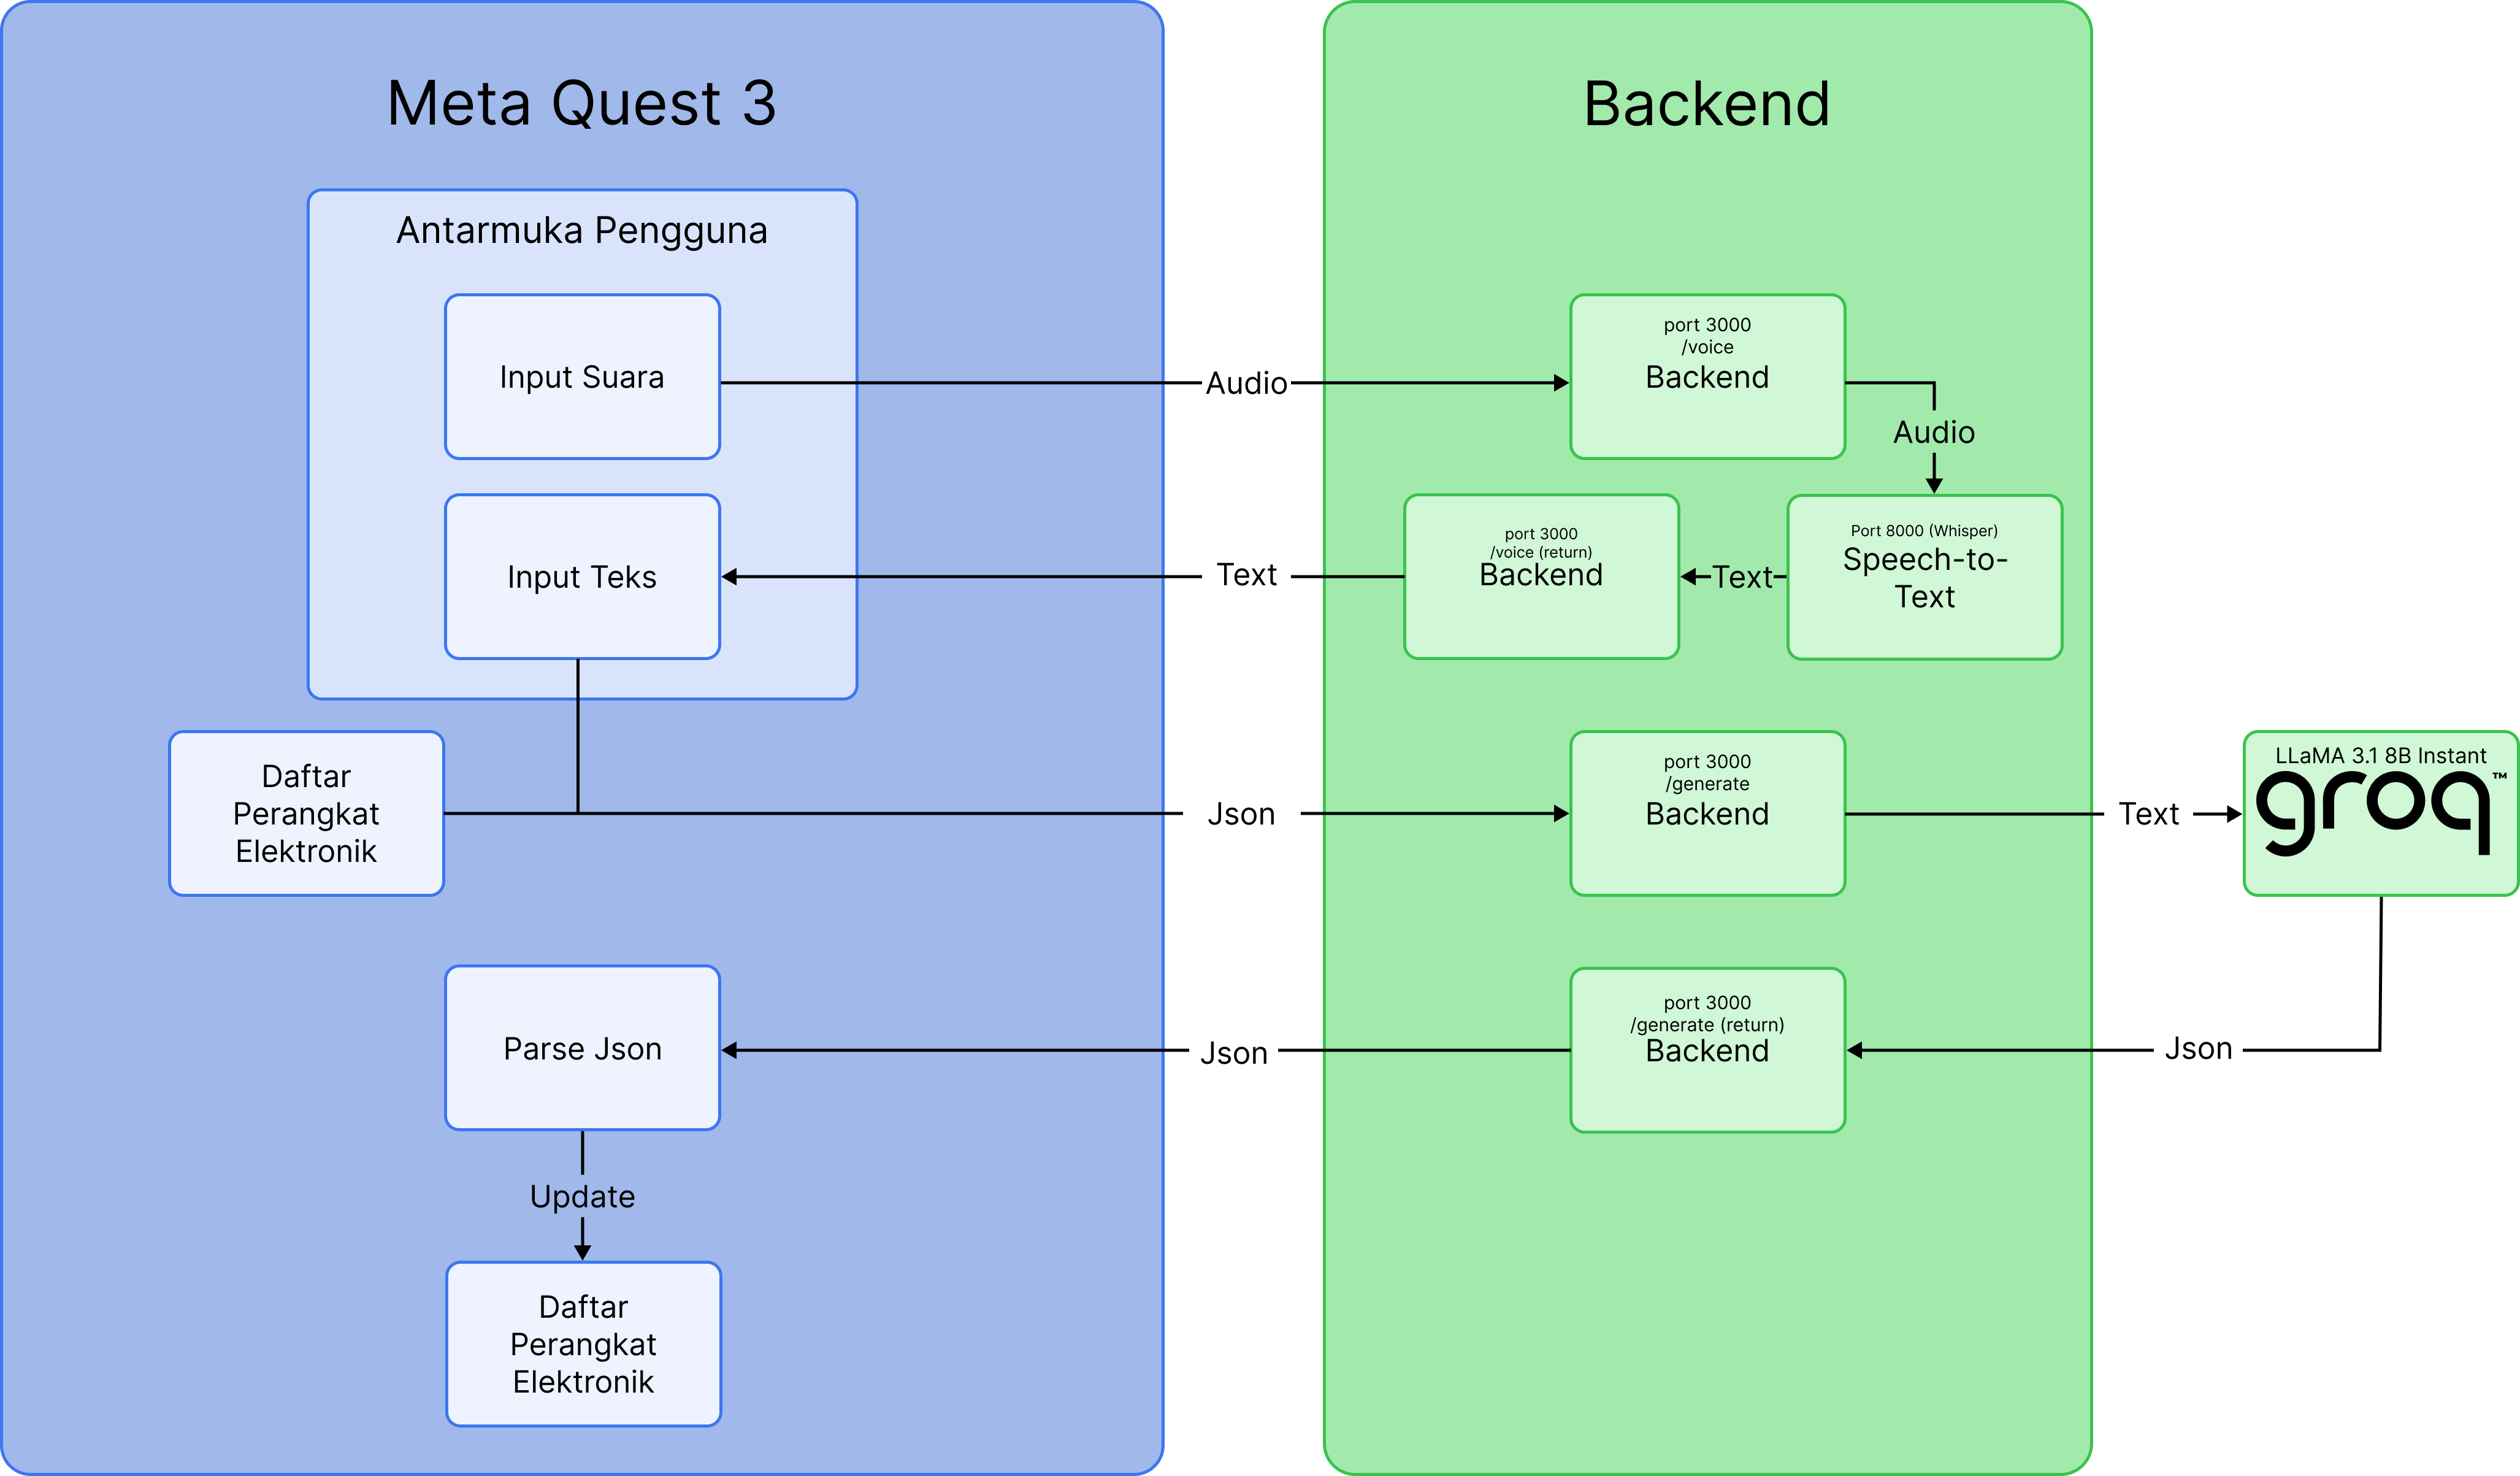
\includegraphics[width=\columnwidth]{arsitektur-sistem.png}}
\caption{ModXplore system architecture.}
\label{fig:arsitektur}
\end{figure}

\subsection{Energy Simulation Module}

Energy estimation follows the Bottom-Up Appliance Modeling approach. Each virtual appliance is assigned a rated power $P$ (W), quantity $n$, and user-configured usage duration $t$ (hours). The energy consumed per appliance type per day is:

\begin{equation}
E = \frac{P \times t \times n}{1000} \quad \text{(kWh)}
\end{equation}

Daily electricity cost is then estimated as:

\begin{equation}
B_{\text{daily}} = E_{\text{total}} \times T
\end{equation}

where $T$ is the applicable electricity tariff (Rp/kWh). Monthly cost accounts for 22 weekdays and 8 weekend days per month:

\begin{equation}
B_{\text{monthly}} = (B_{\text{weekday}} \times 22) + (B_{\text{weekend}} \times 8)
\end{equation}

All parameters — power, quantity, start time, and duration — are configurable by the user through the in-VR interface. The simulation is estimative and does not account for real-time load variations or actual appliance efficiency losses. Fig.~\ref{fig:simulasi} shows the energy estimation panel as displayed inside the VR environment.

\begin{figure}[htbp]
\centerline{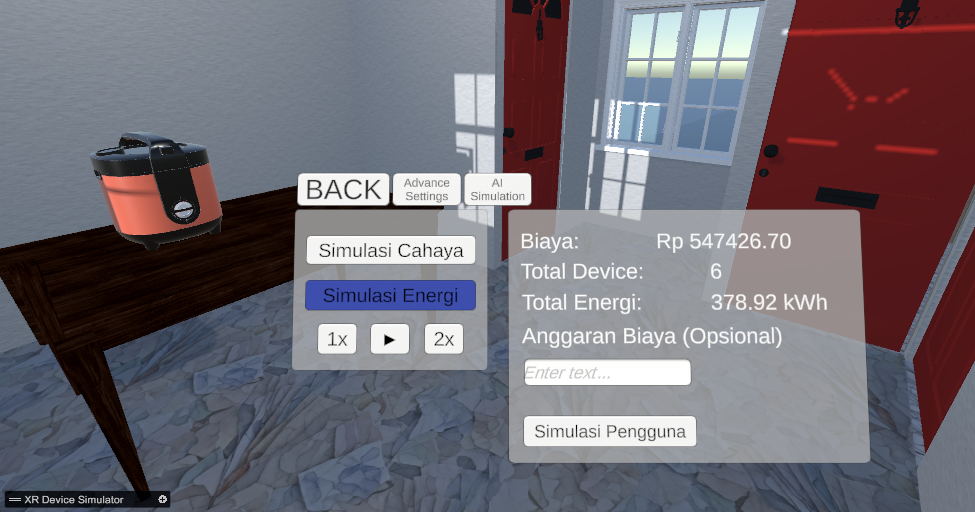
\includegraphics[width=\columnwidth]{simulasi-energi.png}}
\caption{Energy estimation display in the ModXplore VR environment.}
\label{fig:simulasi}
\end{figure}

\subsection{AI-Based Schedule Personalization}

To minimize the manual configuration burden required from users, ModXplore integrates LLaMA 3.1 8B Instant via the Groq API. Users describe their daily routine in natural language — either by text input or by voice transcribed locally via Faster-Whisper. A zero-shot prompt is constructed containing the activity description, the list of available virtual appliances, scheduling rules for weekdays and weekends, and a required JSON output schema. The LLM returns a structured schedule specifying each appliance's start time and usage duration for both day types. The Unity client parses the JSON and applies it to the simulation, instantly updating the energy and cost estimation display. Fig.~\ref{fig:ai} shows the AI-generated schedule result as presented to the user inside the VR application.

\begin{figure}[htbp]
\centerline{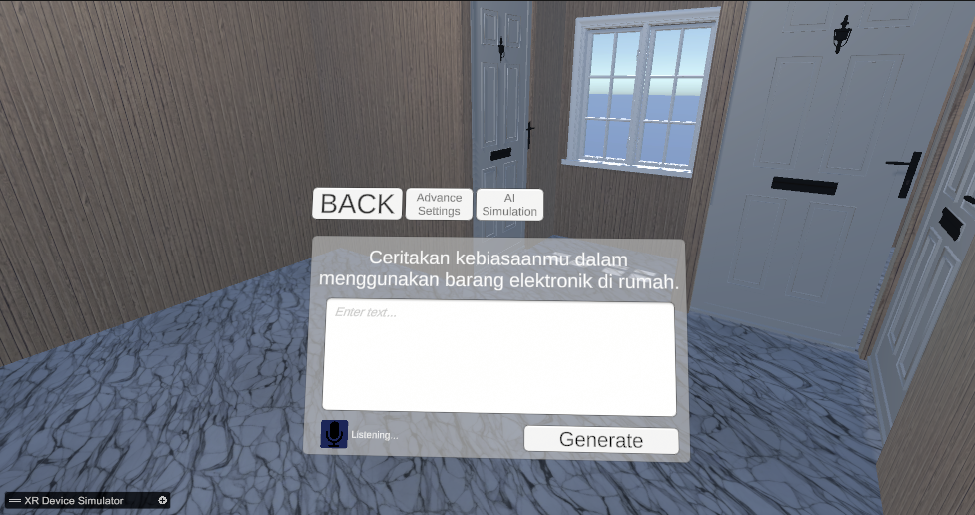
\includegraphics[width=\columnwidth]{ai-schedule.png}}
\caption{AI-generated appliance schedule displayed in ModXplore.}
\label{fig:ai}
\end{figure}

\section{Evaluation}

\subsection{Functional Testing}

Black-box testing was conducted across 29 test scenarios covering all major features: VR house exploration, room navigation, appliance interaction, schedule configuration, energy estimation display, voice input, and AI-generated schedule generation. Each scenario was verified against its expected output. Table~\ref{tab:functional} summarizes the test scenarios by functional category. All 29 scenarios passed without errors, confirming that the implemented features operate as designed within a single integrated VR environment.

\begin{table}[htbp]
\caption{Functional Testing Summary by Category}
\label{tab:functional}
\begin{center}
\begin{tabular}{|p{5cm}|c|c|}
\hline
\textbf{Category} & \textbf{Scenarios} & \textbf{Passed} \\
\hline
VR house exploration and customization (navigation, materials, furniture, doors/windows, lighting, appliance toggling) & 18 & 18 \\
\hline
Energy simulation and AI personalization (appliance configuration, energy/cost estimation, voice input, AI schedule generation) & 11 & 11 \\
\hline
\textbf{Total} & \textbf{29} & \textbf{29} \\
\hline
\end{tabular}
\end{center}
\end{table}

\subsection{User Study}

A user study was conducted with 24 respondents who tested the application as general users. Each participant completed a structured task scenario inside the VR environment, then filled out three evaluation instruments: the System Usability Scale (SUS), the User Experience Questionnaire (UEQ), and a Likert-scale questionnaire (1--5) assessing energy understanding and decision-making support.

The SUS score is computed from ten alternating positive and negative statements, each rated on a 0--4 scale, and converted to a 0--100 scale \cite{brooke1996sus}:

\begin{equation}
SUS = 2.5 \times \sum_{i=1}^{10} x_i
\end{equation}

where $x_i = \text{response}_i - 1$ for odd-numbered (positively worded) items and $x_i = 5 - \text{response}_i$ for even-numbered (negatively worded) items.

For UEQ, each of the six scales (Attractiveness, Perspicuity, Efficiency, Dependability, Stimulation, and Novelty) is scored as the mean of its associated item ratings, where each item is rated on a 7-point scale (1--7) and transformed to a $-3$ to $+3$ range \cite{schrepp2023handbook}:

\begin{equation}
UEQ_{\text{scale}} = \frac{1}{n}\sum_{j=1}^{n}(r_j - 4)
\end{equation}

where $r_j$ is the raw rating of item $j$ and $n$ is the number of items belonging to that scale. The resulting scale means are then compared against the UEQ benchmark dataset.

\section{Results and Discussion}

All 29 functional test scenarios passed as designed. For energy estimation accuracy, two appliance schedule configurations (Default and Energy-Saving) were compared. As shown in Table~\ref{tab:energy}, the Energy-Saving scenario yielded lower consumption on both weekdays and weekends, with a monthly cost difference of 8.48\%, confirming that the Bottom-Up model correctly distinguishes usage patterns.

\begin{table}[htbp]
\caption{Energy Estimation Comparison: Default vs. Energy-Saving Scenario}
\label{tab:energy}
\begin{center}
\begin{tabular}{|l|c|c|c|}
\hline
\textbf{Parameter} & \textbf{Default} & \textbf{Energy-Saving} & \textbf{Difference} \\
\hline
Weekday consumption & 13.40 kWh & 12.38 kWh & 1.02 kWh \\
\hline
Weekend consumption & 14.44 kWh & 12.90 kWh & 1.54 kWh \\
\hline
Monthly cost & Rp592,728 & Rp542,476 & Rp50,252 \\
\hline
Cost difference & \multicolumn{2}{c|}{---} & \textbf{8.48\%} \\
\hline
\end{tabular}
\end{center}
\end{table}

This difference originates from the appliance usage schedules underlying each scenario. Table~\ref{tab:schedule} compares the Default schedule with the schedule generated by the LLM from the activity description \textit{"I am a frugal person"} (Energy-Saving scenario). The AI-generated schedule reduced the usage duration of several appliances, particularly the air conditioner and bedroom lights, while leaving constantly-running appliances such as the refrigerator unchanged. The Bottom-Up Appliance Modeling computation (Eq.~1--3) directly reflects these reduced durations, which is why the Energy-Saving scenario in Table~\ref{tab:energy} consistently yields lower consumption and cost.

\begin{table}[htbp]
\caption{Appliance Schedule Comparison: Default vs. AI-Generated (Energy-Saving)}
\label{tab:schedule}
\begin{center}
\begin{tabular}{|l|c|c|c|c|}
\hline
\multirow{2}{*}{\textbf{Appliance}} & \multicolumn{2}{c|}{\textbf{Default}} & \multicolumn{2}{c|}{\textbf{AI-Generated}} \\
\cline{2-5}
 & \textbf{Weekday} & \textbf{Weekend} & \textbf{Weekday} & \textbf{Weekend} \\
\hline
Refrigerator & 00:00, 24h & 00:00, 24h & 00:00, 24h & 00:00, 24h \\
\hline
Air Conditioner & 22:00, 5h & 21:00, 7h & 22:00, \textbf{3h} & 21:00, \textbf{4h} \\
\hline
Living Room Light & 20:00, 4h & 18:00, 6h & 20:00, 4h & 18:00, \textbf{5h} \\
\hline
Bedroom 1 Light & 20:00, 4h & 18:00, 6h & 21:00, \textbf{2h} & 20:00, \textbf{3h} \\
\hline
Bedroom 2 Light & 20:00, 4h & 18:00, 6h & 22:00, \textbf{2h} & 20:00, \textbf{3h} \\
\hline
Bathroom Light & 07:00, 1h & 07:00, 1h & 07:00, 1h & 07:00, 1h \\
\hline
\end{tabular}
\end{center}
\end{table}

A six-item Likert-scale questionnaire (Q1--Q6) was used to measure users' understanding of the energy simulation feature, their perception of the AI scheduling feature, and the system's support for decision-making. Results are shown in Table~\ref{tab:likert-energy}. All six items scored above 4.4 (Strongly Agree), with the hourly energy graph (Q3 = 4.71) and the AI scheduling feature (Q5 = 4.75) receiving the highest ratings, indicating that the visual representation of hourly consumption patterns and the AI-based schedule recommendation were especially effective. Fig.~\ref{fig:grafik} shows the hourly energy consumption graph as displayed in the VR environment.

\begin{table}[htbp]
\caption{User Evaluation Questionnaire Results (Q1--Q6)}
\label{tab:likert-energy}
\begin{center}
\begin{tabular}{|c|p{5.5cm}|c|}
\hline
\textbf{Item} & \textbf{Statement} & \textbf{Mean} \\
\hline
Q1 & Helps understand appliance energy consumption & 4.54 \\
\hline
Q2 & Gives a clear picture of electricity bill estimation & 4.58 \\
\hline
Q3 & Hourly graph helps understand usage patterns & 4.71 \\
\hline
Q4 & Helps consider energy efficiency when choosing appliances & 4.50 \\
\hline
Q5 & AI feature eases configuration of an energy-saving schedule & 4.75 \\
\hline
Q6 & Supports better decisions on electricity usage & 4.54 \\
\hline
\end{tabular}
\end{center}
\end{table}

\begin{figure}[htbp]
\centerline{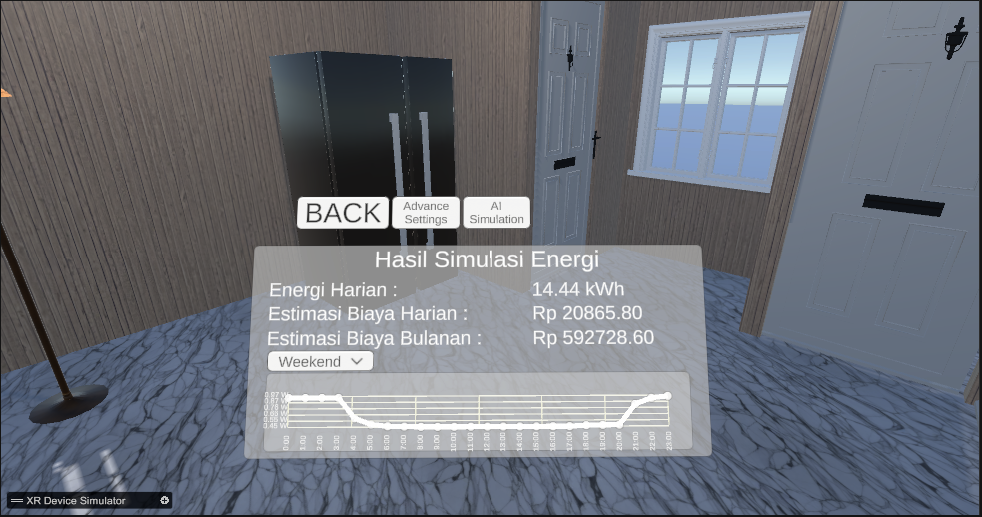
\includegraphics[width=\columnwidth]{grafik-energi.png}}
\caption{Hourly electricity consumption graph in ModXplore.}
\label{fig:grafik}
\end{figure}

The SUS evaluation yielded an average score of 71.56 (Grade C+, 60th--64th percentile on the Sauro--Lewis Curved Grading Scale), indicating an acceptable usability level. Individual scores ranged from 57.5 to 87.5, showing some variability in how easily respondents adapted to the VR interface. The UEQ results per scale are shown in Table~\ref{tab:ueq}. Five of six scales reached the \textit{Excellent} benchmark; only \textit{Perspicuity} was rated \textit{Good} (1.91), reflecting that VR interaction was relatively unfamiliar for some respondents. This is consistent with the SUS variability noted above, suggesting that initial VR learnability, rather than the energy simulation or AI scheduling features themselves, was the primary factor behind lower individual scores.

\begin{table}[htbp]
\caption{UEQ Evaluation Results per Scale}
\label{tab:ueq}
\begin{center}
\begin{tabular}{|l|c|c|}
\hline
\textbf{Scale} & \textbf{Mean} & \textbf{Benchmark} \\
\hline
Attractiveness  & 2.25 & \textit{Excellent} \\
Perspicuity     & 1.91 & \textit{Good} \\
Efficiency      & 2.16 & \textit{Excellent} \\
Dependability   & 2.05 & \textit{Excellent} \\
Stimulation     & 2.25 & \textit{Excellent} \\
Novelty         & 2.30 & \textit{Excellent} \\
\hline
\textbf{Overall} & \textbf{2.15} & --- \\
\hline
\end{tabular}
\end{center}
\end{table}

All six items in Table~\ref{tab:likert-energy} achieved a mean score above 4.4, falling into the Strongly Agree category. These results confirm that users found the system effective in supporting energy understanding, AI-based schedule configuration, and energy-efficient decision-making.

Table~\ref{tab:comparison} compares ModXplore against the most closely related prior work \cite{skripsikating}, which also used Unity and Meta Quest 3 for VR house design. ModXplore extends that foundation with three new capabilities — appliance-level energy simulation, daily/monthly kWh estimation, and AI-based schedule personalization — while maintaining a higher SUS grade (C+ vs. C). This confirms that the added functional complexity did not degrade usability.

\begin{table}[htbp]
\caption{Feature and Usability Comparison with Prior Work}
\label{tab:comparison}
\begin{center}
\begin{tabular}{|p{3.5cm}|c|c|}
\hline
\textbf{Feature} & \textbf{Suryanto \cite{skripsikating}} & \textbf{ModXplore} \\
\hline
VR house exploration        & \checkmark & \checkmark \\
\hline
Material customization      & \checkmark & \checkmark \\
\hline
Furniture placement         & \checkmark & \checkmark \\
\hline
Energy consumption simulation & $\times$ & \checkmark \\
\hline
Daily/monthly kWh estimation  & $\times$ & \checkmark \\
\hline
AI schedule personalization   & $\times$ & \checkmark \\
\hline
Respondents                 & 28    & 24 \\
\hline
SUS score                   & 70.63 & 71.56 \\
\hline
SUS grade                   & C     & C+ \\
\hline
\end{tabular}
\end{center}
\end{table}

A per-scale UEQ comparison with \cite{skripsikating} is shown in Table~\ref{tab:ueq-comparison}. Four of six scales improved, with \textit{Efficiency} rising from \textit{Good} (1.82) to \textit{Excellent} (2.16) and \textit{Perspicuity} rising from \textit{Above Average} (1.61) to \textit{Good} (1.91), indicating that the interface remained efficient and became easier to learn despite the added functionality. The largest gain was in \textit{Novelty} (1.96 to 2.30), suggesting that the energy simulation and AI scheduling features were perceived as a strong novel contribution. \textit{Attractiveness} showed a small decrease (2.34 to 2.25), though both remain in the \textit{Excellent} category; this difference may be attributable to differing respondent characteristics between the two studies rather than a functional regression.

\begin{table}[htbp]
\caption{UEQ Per-Scale Comparison with Prior Work}
\label{tab:ueq-comparison}
\begin{center}
\begin{tabular}{|l|c|c|}
\hline
\textbf{Scale} & \textbf{Suryanto \cite{skripsikating}} & \textbf{ModXplore} \\
\hline
Attractiveness  & 2.34 (Excellent)     & 2.25 (Excellent) \\
\hline
Perspicuity     & 1.61 (Above Average) & 1.91 (Good) \\
\hline
Efficiency      & 1.82 (Good)          & 2.16 (Excellent) \\
\hline
Dependability   & 2.00 (Excellent)     & 2.05 (Excellent) \\
\hline
Stimulation     & 2.11 (Excellent)     & 2.25 (Excellent) \\
\hline
Novelty         & 1.96 (Excellent)     & 2.30 (Excellent) \\
\hline
\end{tabular}
\end{center}
\end{table}

These findings suggest that immersive VR combined with appliance-level energy feedback and AI-assisted scheduling is an effective approach for improving household energy literacy. The UEQ benchmark comparison is further illustrated in Fig.~\ref{fig:ueq}.

\begin{figure}[htbp]
\centerline{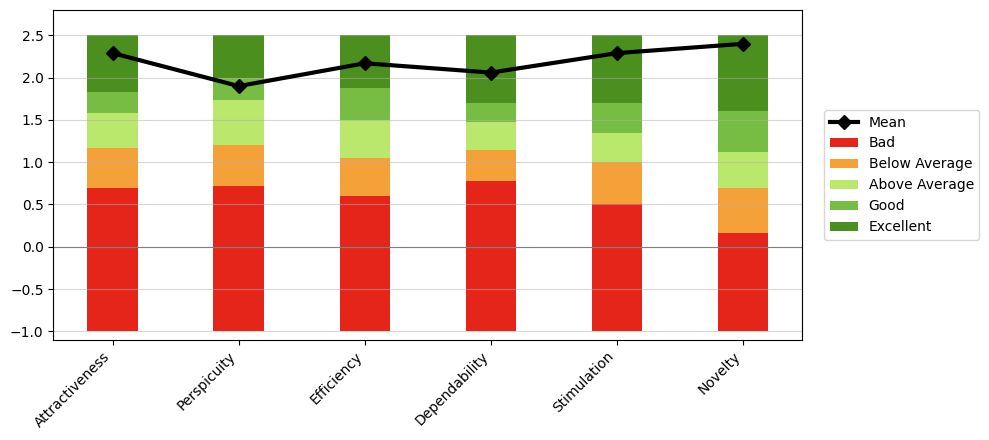
\includegraphics[width=\columnwidth]{ueq-benchmark.png}}
\caption{UEQ benchmark comparison results for ModXplore.}
\label{fig:ueq}
\end{figure}

A few threats to validity should also be noted. First, the user study involved 24 respondents who acted as general users rather than confirmed prospective homeowners, which may not fully capture the priorities of users actively planning a home purchase or construction. Second, the energy estimation comparison (Table~\ref{tab:energy}) was evaluated on a single house design (Type 36 Model 2) with a fixed appliance configuration; results may vary for other house types or appliance sets. Third, the Bottom-Up Appliance Modeling approach assumes constant rated power and does not account for real-time load variation, appliance efficiency degradation, or standby consumption. Finally, the AI-based schedule personalization relies on an external LLM API (Groq), whose output quality and response time may vary depending on network conditions and prompt phrasing, which were not systematically varied in this study.

\section{Conclusion}

This paper presented ModXplore, an interactive VR-based simulation system that integrates immersive house exploration, Bottom-Up Appliance Modeling for household electricity estimation, and LLM-based schedule personalization on Meta Quest 3. The system was evaluated through functional testing and a user study with 24 respondents. Results showed that all features performed correctly, the energy estimation module accurately differentiated usage scenarios (8.48\% monthly cost difference), usability was acceptable (SUS = 71.56), and user experience was rated Excellent on five of six UEQ scales. Users also reported strong support for energy understanding and decision-making. Future work should address the limitations discussed above by validating the system with prospective homeowners, testing across multiple house designs, and applying the system to larger respondent groups for broader generalizability.

\section*{Acknowledgment}

The authors would like to thank all 24 respondents who participated in the user study for their time and valuable feedback.

%Please number citations consecutively within brackets \cite{b1}. The 
%sentence punctuation follows the bracket \cite{b2}. Refer simply to the reference 
%number, as in \cite{b3}---do not use ``Ref. \cite{b3}'' or ``reference \cite{b3}'' except at 
%the beginning of a sentence: ``Reference \cite{b3} was the first $\ldots$''
%
%Number footnotes separately in superscripts. Place the actual footnote at 
%the bottom of the column in which it was cited. Do not put footnotes in the 
%abstract or reference list. Use letters for table footnotes.
%
%Unless there are six authors or more give all authors' names; do not use 
%``et al.''. Papers that have not been published, even if they have been 
%submitted for publication, should be cited as ``unpublished'' \cite{b4}. Papers 
%that have been accepted for publication should be cited as ``in press'' \cite{b5}. 
%Capitalize only the first word in a paper title, except for proper nouns and 
%element symbols.
%
%For papers published in translation journals, please give the English 
%citation first, followed by the original foreign-language citation \cite{b6}.



\bibliography{references}{}
\bibliographystyle{IEEEtran}

%\begin{thebibliography}{00}
%\bibitem{b1} G. Eason, B. Noble, and I. N. Sneddon, ``On certain integrals of Lipschitz-Hankel type involving products of Bessel functions,'' Phil. Trans. Roy. Soc. London, vol. A247, pp. 529--551, April 1955.
%\bibitem{b2} J. Clerk Maxwell, A Treatise on Electricity and Magnetism, 3rd ed., vol. 2. Oxford: Clarendon, 1892, pp.68--73.
%\bibitem{b3} I. S. Jacobs and C. P. Bean, ``Fine particles, thin films and exchange anisotropy,'' in Magnetism, vol. III, G. T. Rado and H. Suhl, Eds. New York: Academic, 1963, pp. 271--350.
%\bibitem{b4} K. Elissa, ``Title of paper if known,'' unpublished.
%\bibitem{b5} R. Nicole, ``Title of paper with only first word capitalized,'' J. Name Stand. Abbrev., in press.
%\bibitem{b6} Y. Yorozu, M. Hirano, K. Oka, and Y. Tagawa, ``Electron spectroscopy studies on magneto-optical media and plastic substrate interface,'' IEEE Transl. J. Magn. Japan, vol. 2, pp. 740--741, August 1987 [Digests 9th Annual Conf. Magnetics Japan, p. 301, 1982].
%\bibitem{b7} M. Young, The Technical Writer's Handbook. Mill Valley, CA: University Science, 1989.
%\end{thebibliography}



\end{document}
